\documentclass[aps,pra,twocolumn,superscriptaddress,nofootinbib]{revtex4-2}
\usepackage{amsmath,amssymb,amsthm}
\usepackage{graphicx}
\usepackage{booktabs}
\usepackage{tikz}
\usetikzlibrary{positioning,arrows.meta,shapes.misc}
\usepackage[colorlinks=true,linkcolor=blue!50!black,citecolor=blue!50!black,urlcolor=blue!50!black]{hyperref}

\newtheorem{theorem}{Theorem}
\newtheorem{lemma}{Lemma}
\input{generated/macros.tex}

\newcommand{\ket}[1]{|#1\rangle}
\newcommand{\bra}[1]{\langle#1|}
\newcommand{\norm}[1]{\lVert#1\rVert}

\begin{document}

\title{From classical energy estimates to a certified ground state:\\
a modular Stetcu--Baroni filter pipeline and its cost for the $J_1$--$J_2$ chain}

\author{Authors to be added}
\date{\today}

\begin{abstract}
Classical methods such as the density-matrix renormalization group (DMRG) supply accurate
ground-state energies, a gap estimate and a compact trial state, but a shallow circuit for that trial
state keeps some weight on excited states. The projection filter of Stetcu, Baroni and Carlson removes
it with one ancilla, controlled time evolution and post-selection. We give a generic, modular pipeline
that takes energy estimates and an ansatz for any Hamiltonian written as a sum of Pauli strings, designs
a cosine filter with a certified suppression ratio, chooses first- or second-order Trotter step counts
from commutator bounds, and returns an a-priori bound on the infidelity of the prepared state together
with a transparent gate count. The bound is a theorem conditional on the inputs (an interval for the
ground energy, a lower bound on the gap and on the trial overlap), and every one of these conditions is
an explicit input. We apply it to the open spin-$\tfrac12$ $J_1$--$J_2$ chain with DMRG inputs and
bond-dimension-$\chi$ matrix-product trial states, $N=8$--$48$. In all \nSimOK{} of \nSim{} simulated
circuits ($N\le14$) the certified bound held; it overestimates the measured infidelity by a median
factor of \boundRatioMed, mostly through its Trotter term. A second-order product formula is a median
\gainOrderMed$\times$ cheaper than first order, and an optimized filter a median \gainOptMed$\times$
cheaper than a closed-form halving (``dyadic'') schedule, which however is the only design that stays
feasible for small overlaps. Near the critical coupling at $N=48$, a $\chi=4$ trial state is refined to
infidelity $10^{-2}$ for \cnotFortyEightChiFour{} CNOTs per success. Overestimating the gap by
$50\%$ is the one input error that broke the target; a conservative gap costs at most
\gapMarginCost$\times$. For this one-dimensional model at $\epsilon=10^{-2}$, however, a $\chi=8$
matrix-product circuit alone already meets the target with about $10^{3}$--$10^{4}$ CNOTs, so the value of
the pipeline lies in its certificate and in models where compact trial states are not available.
\end{abstract}

\maketitle

%=====================================================================================================
\section{Introduction}

A common route to a ground state on a quantum computer starts classically: an approximate method
produces a trial state that can be compiled into a short circuit, and a quantum subroutine removes its
residual excited-state weight. For one-dimensional and quasi-one-dimensional systems the natural
classical engine is DMRG~\cite{White1992,Schollwock2011}, which yields the ground-state energy $E_0$,
excited-state energies and a matrix-product state (MPS) whose low-bond-dimension truncations compile
exactly into staircase circuits~\cite{Ran2020}. The quantum step can be phase estimation~\cite{Ge2019},
a polynomial filter implemented by quantum singular-value
transformation~\cite{Lin2020,Gilyen2019,Dong2022}, or a product of cosine filters implemented with a
single ancilla~\cite{Stetcu2023,Choi2021}. The last option, the projection algorithm of Stetcu, Baroni
and Carlson (SBC)~\cite{Stetcu2023}, is attractive for early fault-tolerant hardware: each step is one
controlled time evolution sandwiched between ancilla rotations and a measurement, the filter is
designed classically, and the success probability is known in advance.

To use such a filter one has to answer three practical questions: which times and phases, how many
Trotter steps, and how good the result is. SBC optimize the times and phases numerically for a model
spectrum with a given gap; they do not give a bound on the error of the prepared state, and the
Trotter error is treated separately~\cite{Stetcu2023}. This paper packages the full chain as a pipeline
with typed inputs and a certificate:
\begin{enumerate}
\item \emph{Inputs}: a Pauli-sum Hamiltonian $H$, energy estimates (an interval for $E_0$, a lower
  bound on the first excited energy $E_1$, optionally an upper bound on the spectrum) and an ansatz
  (its estimated ground-space weight $\gamma$ and the gate cost of its circuit). Any classical method
  can supply them.
\item \emph{Filter design}: three schedules, from the naive repeated cosine to an optimized design,
  each with a rigorous interval bound on its suppression ratio.
\item \emph{Trotterization}: first- and second-order commutator-scaling bounds~\cite{Childs2021},
  evaluated exactly on the support of each local commutator.
\item \emph{Certificate}: an a-priori bound on the trace distance between the prepared state and the
  ground space, valid whenever the inputs are valid.
\item \emph{Resources}: qubits, CNOTs, arbitrary rotations, a $T$-count estimate and the expected cost
  per successful preparation.
\end{enumerate}
We then apply it to the open $J_1$--$J_2$ Heisenberg chain using DMRG, validate the certificate by
statevector simulation for $N\le14$, and report resources for $N\le48$. The code is the \texttt{sbpipe}
package, available with all data at \url{https://github.com/aaronseymour7/FilterPipeline}; every number below is produced by the scripts named in
Appendix~\ref{app:repro}.

The contribution is methodological and quantitative rather than algorithmic: the filter is SBC's, the
Trotter bounds are those of Childs \emph{et al.}~\cite{Childs2021}, and the certificate follows the
standard triangle-inequality argument. What is new is a generic interface whose guarantees are stated
in terms of the inputs, a closed-form ``dyadic'' energy schedule with $O(\Delta^{-1}\log\eta^{-1})$
total time, and a calibrated account of what this costs and where the bound is loose for a concrete,
physically relevant model.

%=====================================================================================================
\section{The pipeline}
\label{sec:pipeline}

\begin{figure}[t]
\centering
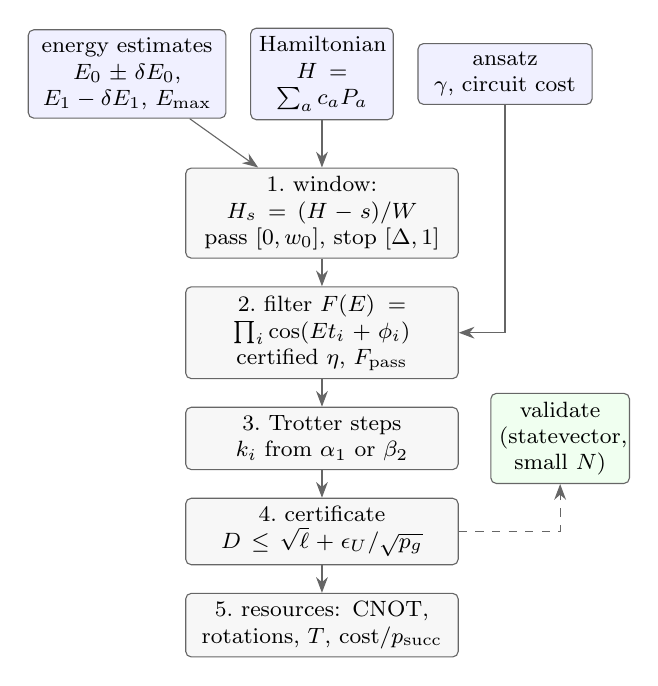
\begin{tikzpicture}[node distance=3.5mm and 3mm, font=\footnotesize,
  box/.style={draw=black!60, rounded corners=2pt, align=center, inner sep=3pt, minimum height=7mm},
  inp/.style={box, fill=blue!6}, stage/.style={box, fill=black!3, text width=3.25cm},
  arr/.style={-{Stealth[length=2mm]}, black!60}]
\node[inp, text width=2.3cm] (E) {energy estimates\\$E_0\pm\delta E_0$, $E_1-\delta E_1$, $E_{\max}$};
\node[inp, text width=1.6cm, right=of E] (H) {Hamiltonian\\$H=\sum_a c_aP_a$};
\node[inp, text width=2.0cm, right=of H] (A) {ansatz\\$\gamma$, circuit cost};
\node[stage, below=6mm of H] (W) {1.~window: $H_s=(H-s)/W$\\ pass $[0,w_0]$, stop $[\Delta,1]$};
\node[stage, below=of W] (D) {2.~filter $F(E)=\prod_i\cos(Et_i+\phi_i)$\\certified $\eta$, $F_{\rm pass}$};
\node[stage, below=of D] (T) {3.~Trotter steps $k_i$ from $\alpha_1$ or $\beta_2$};
\node[stage, below=of T] (C) {4.~certificate $D\le\sqrt{\ell}+\epsilon_U/\sqrt{p_g}$};
\node[stage, below=of C] (R) {5.~resources: CNOT, rotations, $T$, cost$/p_{\rm succ}$};
\node[box, fill=green!6, right=4mm of T, text width=1.55cm] (V) {validate\\(statevector, small $N$)};
\draw[arr] (E) -- (W); \draw[arr] (H) -- (W); \draw[arr] (A.south) |- (D.east);
\draw[arr] (W) -- (D); \draw[arr] (D) -- (T); \draw[arr] (T) -- (C); \draw[arr] (C) -- (R);
\draw[arr, dashed] (C.east) -| (V.south);
\end{tikzpicture}
\caption{The pipeline. Blue: inputs, which any classical method can supply. Grey: the stages of
\texttt{refine()}. Green: the optional statevector check used in Sec.~\ref{sec:validation}.}
\label{fig:workflow}
\end{figure}

\subsection{Inputs and the spectral window}

The Hamiltonian is $H=\sum_a c_aP_a$ with real $c_a$ and Pauli strings $P_a$, in a fixed order that is
also the Trotter order, and with an optional grouping of terms (here: one group per bond). The pipeline
assumes
\begin{equation}
\begin{gathered}
E_0\in[E_0^{\rm est}-\delta E_0,\;E_0^{\rm est}+\delta E_0],\\
E_1\ge E_1^{\rm est}-\delta E_1,\qquad E_{\rm top}\le E_{\max},
\end{gathered}
\label{eq:assumptions}
\end{equation}
where $E_1$ is the lowest level above the ground space that the trial state can overlap with. If no
$E_{\max}$ is given, the Weyl bound $E_{\max}=\sum_g\lambda_{\max}(h_g)$ over the term groups $h_g$ is
used; it is rigorous and, for the antiferromagnetic $J_1$--$J_2$ chain, attained by the ferromagnetic
state. With $s=E_0^{\rm est}-\delta E_0$ and $W=E_{\max}-s$, the scaled Hamiltonian $H_s=(H-s)/W$ has its
ground energy in the \emph{pass band} $[0,w_0]$, $w_0=2\delta E_0/W$, and every other relevant level in
the \emph{stop band} $[\Delta,1]$, $\Delta=(E_1^{\rm est}-\delta E_1-s)/W$.

The ansatz enters through $\gamma$, a lower estimate of its weight on the ground space, and through the
gate cost of the circuit that prepares it. A statevector is needed only for validation.

\subsection{The filter and three schedules}

One SBC pulse~\cite{Stetcu2023} applies $\mathsf H_a\,e^{-itH_s\otimes Z_a}\,R_z^{(a)}(2\phi)\,\mathsf H_a$
to the system and an ancilla in $\ket0$; the ancilla-$\ket0$ block of this unitary is
$\cos(H_st+\phi)$. (SBC write the same block with $e^{-i(tH+\delta)\otimes Y_a}$.) Keeping outcome 0
after $m$ pulses applies
\begin{equation}
F(H_s)=\prod_{i=1}^m\cos(H_st_i+\phi_i),\qquad T=\sum_i|t_i|.
\end{equation}
Two numbers characterize a filter: the pass-band floor $F_{\rm pass}\le\min_{[0,w_0]}|F|$ and the
suppression ratio $\eta=\sup_{[\Delta,1]}|F|/F_{\rm pass}$. Both are certified, not sampled: since
$|F'|\le L:=\sum_i|t_i|$ and $|F''|\le L^2$, an interval branch-and-bound gives a rigorous upper bound
on $\sup|F|$ over the stop band, and $F_{\rm pass}=|F(0)|-Lw_0$ (the certifier is
\texttt{sbpipe.floor.certify}; it is used for the optimized schedule, the other two have
closed-form certificates). Given a target leakage $\epsilon_\ell$ and $\gamma$, the
design target is $\eta^2\le\gamma\epsilon_\ell/[(1-\epsilon_\ell)(1-\gamma)]$ (Lemma~\ref{lem:leak}).
We provide three schedules:

\emph{Uniform}: $m$ equal pulses $t=\pi/(1+\Delta)$, $\phi=0$, so $F=\cos^m(Et)$ and
$\sup_{[\Delta,1]}|\cos Et|=\cos\theta$, $\theta=\pi\Delta/(1+\Delta)$. Then
$m\approx2\ln(1/\eta)/\theta^2$ and $T\approx2\ln(1/\eta)/(\pi\Delta^2)$: quadratic in the inverse gap.
It is the baseline that any design should beat.

\emph{Dyadic}: $r$ repetitions of the halving ladder $t=\tau,2\tau,\dots,2^{K-1}\tau$,
$\tau=\pi/(1+\Delta)$, $\phi=0$. This is the schedule SBC use for quantum-number
projection~\cite{Stetcu2023}, here applied to the energy. One block is a Dirichlet kernel,
\begin{equation}
\prod_{k=0}^{K-1}\cos(2^kE\tau)=\frac{\sin(2^KE\tau)}{2^K\sin(E\tau)},
\label{eq:dirichlet}
\end{equation}
which equals 1 at $E=0$ and is at most $\eta_b=1/(2^K\sin\theta)$ on $[\Delta,1]$ because
$\sin(E\tau)\ge\sin\theta$ there. With $r=\lceil\ln\eta/\ln\eta_b\rceil$ blocks,
$T=r\tau(2^K-1)$; choosing $2^K\sin\theta\approx e$ gives
\begin{equation}
T_{\rm dyadic}\approx\frac{e\,\tau}{\sin\theta}\ln\frac1\eta\;\approx\;\frac{e}{\Delta}\ln\frac1\eta ,
\end{equation}
the optimal $O(\Delta^{-1}\log\eta^{-1})$ scaling~\cite{Lin2020} with an explicit constant and no
optimization. The pipeline searches $K$ and $r$ for the smallest $T$. Both closed-form schedules are
certified by the inequalities just given (with $F_{\rm pass}=\cos^m(w_0t)$ and $1-Lw_0$,
respectively), which avoids interval arithmetic on filters with $L\sim10^{3}$--$10^{5}$; the
test suite checks them against a $2\times10^6$-point grid.

\emph{Optimized}: times and phases chosen to maximize $F(0)^2$ subject to the certified constraint on
$\eta$ at fixed $(T,m)$, over a grid of $x=T\Delta/\pi$ and $m\in\{4,6,8\}$, picking the pair with the
smallest $T^2/F(0)^2$. This is SBC's recipe for energy filters~\cite{Stetcu2023} with a certified
constraint in place of a grid objective; it uses the SLSQP designer \texttt{sbpipe/floor.py}.
Nonzero phases trade success probability ($F(0)<1$) for a shorter $T$.

For each schedule the leakage share $\epsilon_\ell/\epsilon\in\{0.5,0.25,0.1,0.05\}$ is scanned and the
plan with the smallest expected CNOT count per success is kept. An ``auto'' mode does the same over the dyadic and optimized
schedules together.

\subsection{Trotterization}

Each controlled evolution $e^{-it_iH_s\otimes Z_a}$ is approximated by $k_i$ steps of the first-order
(Lie) or second-order (Strang) product formula over the non-identity terms; the identity term of $H_s$
becomes a single ancilla $R_z$ per pulse and is exact. For $B_a=\sum_{b>a}H_b$ the bounds of Childs
\emph{et al.}~\cite[Props.~15--16]{Childs2021} are
\begin{align}
\norm{S_1(t)-e^{-itH}}&\le\tfrac{t^2}{2}\alpha_1,&\alpha_1&=\textstyle\sum_a\norm{[B_a,H_a]},\\
\norm{S_2(t)-e^{-itH}}&\le t^3\beta_2,&\beta_2&=\textstyle\frac1{12}\sum_a\norm{[B_a,[B_a,H_a]]}\nonumber\\
&&&\quad+\textstyle\frac1{24}\sum_a\norm{[H_a,[H_a,B_a]]},
\end{align}
so $k$ steps over time $t$ cost $\alpha_1t^2/(2k)$ or $\beta_2t^3/k^2$. Tensoring every term with
$Z_a$ leaves $\alpha_1$ and $\beta_2$ unchanged because $Z_a^2=1$. For Pauli strings
$[P_b,P_a]=2P_bP_a$ when they anticommute and 0 otherwise, so each commutator is a short Pauli sum
supported on a few qubits around term $a$; we evaluate its norm exactly on that support (dense for
$\le8$ qubits, Lanczos up to 12, triangle inequality beyond, which never occurred here). The
constants are maximized over the forward and reversed term order, so they hold for either convention.
A common step size, $k_i=\lceil t_i/\delta t\rceil$, minimizes $\sum_ik_i$ for both orders at a given
error budget (a Lagrange argument), and leaves the certified times untouched.

\subsection{The certificate}

\begin{theorem}\label{thm:cert}
Assume \eqref{eq:assumptions} and that the trial state has ground-space weight at least $\gamma$. Let
the designed filter have certified $\eta$ and $F_{\rm pass}$, let $\epsilon_U$ bound the operator-norm
error of the implementation (Trotter error $\sum_i\epsilon_i$ plus $R\delta$ for the $R$ arbitrary
rotations of the trial and filter circuits, each synthesized to accuracy $\delta$), and let
\begin{equation}
\ell=\frac{(1-\gamma)\eta^2}{\gamma+(1-\gamma)\eta^2},\qquad p_g=\gamma F_{\rm pass}^2 .
\end{equation}
Then, conditioned on the ancilla outcomes 0, the prepared state $\tilde\rho$ satisfies
\begin{equation}
D(\tilde\rho,\Pi_0)\le\sqrt\ell+\frac{\epsilon_U}{\sqrt{p_g}},\qquad 1-F\le D^2,
\label{eq:cert}
\end{equation}
where $D$ is the trace distance to the normalized projection of the trial state on the ground space,
$\langle H\rangle-E_0\le(E_{\rm top}-E_0)D^2$, and the success probability is at least
$(\sqrt{p_g}-\epsilon_U)^2$.
\end{theorem}

The proof (Appendix~\ref{app:proof}) combines a leakage lemma for the exact filter with the
observation that a vector error $\epsilon_U$ on an unnormalized vector of norm at least $\sqrt{p_g}$
moves its direction by at most $\epsilon_U/\sqrt{p_g}$. The pipeline sets the budget
$\epsilon_U\le(\sqrt\epsilon-\sqrt\ell)\sqrt{p_g}$, gives $90\%$ of it to the product formula and the
rest to rotation synthesis. If the trial state already satisfies $1-\gamma\le\epsilon$, the pipeline
also offers the empty filter ($\eta=1$, no post-selection, $\ell=1-\gamma$) and keeps whichever plan
is cheaper.

\subsection{Resource model}

All-to-all connectivity and the Clifford+$R_z$ gate set are assumed. A term $cP\otimes Z_a$ with
$|P|=w$ is a weight-$(w+1)$ Pauli rotation: $2w$ CNOTs in a ladder and one $R_z$. A Lie step costs one
rotation per term; $k$ Strang steps cost $k(2\Gamma-2)+1$ rotations for $\Gamma$ terms because the two
middle half-steps and the outer half-steps of adjacent steps merge. Each pulse adds one ancilla $R_z$.
An arbitrary rotation at accuracy $\delta$ costs $3\log_2(1/\delta)$ $T$ gates, the leading term of
Ross--Selinger synthesis~\cite{Ross2016}. The cost of one attempt is the trial circuit plus the
filter, and the expected cost per success is the attempt cost divided by the success probability,
which we bound below by $p_g$ (repeat-until-success; an early-abort protocol that measures after each
pulse would be cheaper and is not modeled). The ladder CNOT count is an upper bound: qiskit's
synthesis shares CNOTs between the $XX$, $YY$, $ZZ$ terms of a bond and needs 8 instead of 12 per
controlled bond per Lie step (checked in the test suite), so CNOT numbers below can be read as upper
bounds that a compiler lowers by about one third.

%=====================================================================================================
\section{Application: $J_1$--$J_2$ chain with DMRG}
\label{sec:application}

\subsection{Model and front end}

We study the open spin-$\frac12$ chain
\begin{equation}
H=J_1\sum_{i=1}^{N-1}\mathbf S_i\cdot\mathbf S_{i+1}+J_2\sum_{i=1}^{N-2}\mathbf S_i\cdot\mathbf S_{i+2},
\end{equation}
$J_1=1$, at $J_2=0$ (Heisenberg), $J_2=0.2411$ (close to the critical point of the
gapless-to-dimerized transition~\cite{Okamoto1992,Eggert1996}) and $J_2=0.4$ (dimerized), for $N=8$ to
48. Its Pauli form has $3(2N-3)$ terms of weight 2. Terms are ordered by bond: nearest-neighbor bonds
with even then odd left site, then next-nearest-neighbor bonds likewise.

The front end (\texttt{sbpipe/frontends/dmrg\_quimb.py}) builds the MPO from the Pauli sum and runs
two-site DMRG (quimb~\cite{Gray2018}) with bond dimensions up to 256 ($N\le24$) or 128 ($N>24$) and
truncation cutoff $10^{-12}$. $E_1$ is the lowest state of $H+\mu(S^z_{\rm tot}-1)^2$, $\mu=2$, i.e.\
the lowest triplet. The error bars $\delta E_0,\delta E_1$ are the energy change between the last two
bond dimensions, floored at $10^{-10}$; they are convergence heuristics, not bounds. The trial state is
the variationally optimal MPS at fixed bond dimension $\chi\in\{1,2,4,8\}$, and $\gamma$ is its
overlap with the reference MPS. An MPS of bond dimension $2^b$ is exactly a staircase of $N-b$ unitaries
on $b+1$ qubits; we cost each with the quantum Shannon decomposition bound
$\frac{23}{48}4^n-\frac32 2^n+\frac43$ CNOTs (3, 20, 100 for $n=2,3,4$)~\cite{Shende2006} and $4^n-1$
rotations.

For $N\le14$ we compare with exact diagonalization (ED). DMRG reproduces $E_0$ to $\dmrgEzeroErr$,
the first excited level of any symmetry to $\dmrgEoneErr$ (so the first excitation is the triplet in
every ED case, as also found for $N\le16$ in Ref.~\cite{repoWriteup}), and the trial overlaps to
$\dmrgGammaErr$ (largest difference, for a $\chi=1$ trial). The Weyl bound equals the exact top of the spectrum to $\weylErr$.
Table~\ref{tab:inputs} lists the inputs. The trial overlap decays roughly exponentially with $N$ at
fixed $\chi$, the familiar orthogonality catastrophe, so the filter has more to do at larger $N$.

\begin{table}[t]
\caption{DMRG inputs: ground energy, gap $E_1-E_0$ and trial overlap $\gamma$ of the optimal
bond-dimension-$\chi$ MPS. Source: \texttt{results/inputs.json}.}
\label{tab:inputs}
\begin{ruledtabular}
\begin{tabular}{rrrrrrrr}
$N$ & $J_2$ & $E_0$ & gap & $\gamma_{\chi=1}$ & $\gamma_{2}$ & $\gamma_4$ & $\gamma_8$\\
\midrule
\input{generated/tab_inputs.tex}
\end{tabular}
\end{ruledtabular}
\end{table}

\subsection{Validation of the certificate ($N\le14$)}
\label{sec:validation}

For $N\in\{8,10,12,14\}$, the three couplings, $\epsilon\in\{10^{-2},10^{-3}\}$, the three schedules and
both Trotter orders we plan a circuit for the $\chi=2$ trial state and, when its size permits,
simulate it exactly: the ancilla-0 block of the Trotterized circuit is
$\frac12(e^{-i\phi}S(t)+e^{i\phi}S(-t))$ per pulse, applied to the trial statevector and compared with
the ED ground state. Of \nPlans{} plans, \nSim{} were simulated (the others, mostly uniform or first-order plans
with $10^{4}$--$10^{8}$ steps, exceed our simulation budget), and the certificate held in all
\nSimOK{} (Fig.~\ref{fig:validation}).

\begin{figure}[t]
\includegraphics[width=\columnwidth]{figs/fig_validation.pdf}
\caption{All simulated plans. (a) Measured infidelity of the planned circuit divided by the target
$\epsilon$ (the certified bound is $\le\epsilon$ by construction); points are offset horizontally by
schedule and order. (b) Measured distance between the Trotterized and the exact filtered state against
its certified bound. Points below the dashed lines respect the bound. Filled circles: second order;
open squares: first order.}
\label{fig:validation}
\end{figure}

The bound is conservative by a median factor \boundRatioMed{} (range \boundRatioMin--$\boundRatioMax$)
in infidelity. Splitting it shows where: the leakage term $\ell$ overestimates the exact filter's
infidelity by a median \leakRatioMed$\times$ (range \leakRatioMin--$\leakRatioMax$). By schedule the medians are 1.4 (optimized), 4 (uniform)
and 56 (dyadic): the optimized design pushes $|F|$ to $\eta F_{\rm pass}$ across the band, whereas the
closed-form dyadic bound $1/(2^K\sin\theta)$ is reached only near the band edge. More generally, $\eta$ is
a worst case over the whole stop band while the trial state's excited weight sits mostly low in the
band. The
Trotter term overestimates the measured Trotter distance by a median \trotRatioMed$\times$ (range
\trotRatioMin--$\trotRatioMax$), consistent with earlier findings for this model~\cite{repoWriteup}:
commutator bounds are worst-case over all states, while the filtered state lives in the low-energy
subspace, where Trotter errors are much smaller~\cite{Sahinoglu2021}. The measured success probability
equals $p_g$ to two digits in every case, because after filtering almost all of the surviving norm is
ground-state weight.

Table~\ref{tab:schedules} compares the schedules for one case. The uniform filter needs a total time
an order of magnitude larger than the others, as its $\Delta^{-2}$ scaling predicts. The optimized
filter is shortest; its nonzero phases lower $p_g$ (0.58 against 0.81 here), which the cost criterion
accounts for. Second order cuts the step count by one to two orders of magnitude at these sizes.
Figure~\ref{fig:filters} shows the three filter functions.

\begin{figure}[t]
\includegraphics[width=0.95\columnwidth]{figs/fig_filters.pdf}
\caption{$|F(E)|$ of the three schedules for $N=12$, $J_2=0.2411$, $\epsilon=10^{-2}$, second order.
Dotted lines: certified $\eta F_{\rm pass}$. Grey: the gap region. The horizontal axis is linear below
$\Delta$ and logarithmic above.}
\label{fig:filters}
\end{figure}

\begin{table*}[t]
\caption{Plans for $N=12$, $J_2=0.2411$, $\chi=2$ trial. $T_{\rm phys}=T/W$ in units of $1/J_1$; CNOT and
$T$ counts per attempt (filter) and expected per success (trial + filter, divided by $p_g$).
``meas.'': simulated infidelity of the planned circuit. Source: \texttt{results/validate.json}.}
\label{tab:schedules}
\begin{ruledtabular}
\begin{tabular}{rlrrrrrrrrr}
$\epsilon$ & schedule & order & $m$ & $T_{\rm phys}$ & $p_g$ & steps & CNOT (filter) & CNOT/success & $T$/success & meas.\ $1-F$\\
\midrule
\input{generated/tab_schedules.tex}
\end{tabular}
\end{ruledtabular}
\end{table*}

How much of the remaining gap could a better bound recover? For $N\le12$ we bisect a common scale
factor on the certified $k_i$ until the simulated infidelity just meets $\epsilon$. The certified step
count is \oracleMin--\oracleMax$\times$ (median \oracleMed) larger than this oracle value
(Table~\ref{tab:oracle}). The oracle uses the exact ground state and is not a usable rule; it measures
the price of certification at second order.

\begin{table}[t]
\caption{Certified over oracle step count (second order, $\chi=2$). Columns: $N=8,10,12$ for each
$J_2$. Source: \texttt{results/oracle.json}.}
\label{tab:oracle}
\begin{ruledtabular}
\begin{tabular}{llrrrrrrrrr}
 & & \multicolumn{3}{c}{$J_2=0$} & \multicolumn{3}{c}{$J_2=0.2411$} & \multicolumn{3}{c}{$J_2=0.4$}\\
$\epsilon$ & schedule & 8 & 10 & 12 & 8 & 10 & 12 & 8 & 10 & 12\\
\midrule
\input{generated/tab_oracle.tex}
\end{tabular}
\end{ruledtabular}
\end{table}

\subsection{Resources up to $N=48$}

Without simulation the pipeline only needs DMRG, so we plan for $N$ up to 48 with the same $\chi=2$
trial family (Fig.~\ref{fig:scaling}, Table~\ref{tab:scaling}). Over all sizes, couplings and targets
the second-order plan is \gainOrderMin--\gainOrderMax$\times$ (median \gainOrderMed) cheaper than the
first-order plan of the same schedule. The optimized schedule is \gainOptMin--\gainOptMax$\times$
(median \gainOptMed) cheaper than the dyadic one at second order, and more expensive in \nDyaWins{} of
\nOptCmp{} comparable cases. Its numerical design, however, failed in \nScaleFail{} of \nScale{} plans,
all at $N\ge32$ where $\gamma\lesssim0.4$ or $\epsilon=10^{-3}$ demand a suppression $\eta$ the
SLSQP search with $F(0)^2\ge10^{-3}$ did not reach; the dyadic schedule is feasible everywhere, which
is why the pipeline offers an automatic choice between the two. For $N=16$--48 the expected CNOT count
of the dyadic second-order plan grows as $N^{\fitADyaTwoCnot}$, $N^{\fitBDyaTwoCnot}$ and
$N^{\fitCDyaTwoCnot}$ for $J_2=0,0.2411,0.4$, and its step count as $N^{\fitADyaTwoSteps}$,
$N^{\fitBDyaTwoSteps}$, $N^{\fitCDyaTwoSteps}$. These exponents combine the shrinking gap
($T\propto1/\Delta$, and $\Delta=g/W$ with $W\propto N$), the growing commutator constant, the number of
terms per step and the decaying overlap ($1/p_g$); they are fits over $N=16$--48, not asymptotic
statements. At $N=48$, $J_2=0.2411$ the best $\chi=2$ plan (\schedFortyEight) needs
\cnotFortyEight{} CNOTs per success, which the next section reduces by choosing a better trial.

\begin{figure*}[t]
\includegraphics[width=\textwidth]{figs/fig_scaling.pdf}
\caption{Expected CNOTs per successful preparation versus $N$ (trial $\chi=2$, $\epsilon=10^{-2}$),
including the trial circuit and the $1/p_g$ repetitions. Solid: second order; dashed: first order.
Missing optimized points: no feasible design (see text). Source: \texttt{results/scaling.json}.}
\label{fig:scaling}
\end{figure*}

\begin{table*}[t]
\caption{Cheapest second-order plan (``sch.'': dyadic or optimized) for $\epsilon=10^{-2}$, trial
$\chi=2$. $\Delta$ is the scaled gap, $T_{\rm phys}=T/W$ in $1/J_1$. Steps for first (1st) and second
(2nd) order with the same schedule; CNOT and $T$ counts for second order. Source:
\texttt{results/scaling.json}.}
\label{tab:scaling}
\begin{ruledtabular}
\begin{tabular}{rrrrlrrrrrrr}
$N$ & $J_2$ & $\gamma$ & $\Delta$ & sch. & $T_{\rm phys}$ & $p_g$ & steps (1st) & steps (2nd) & CNOT/attempt & CNOT/success & $T$/success\\
\midrule
\input{generated/tab_scaling.tex}
\end{tabular}
\end{ruledtabular}
\end{table*}

\subsection{What if the energy estimates are wrong?}

The certificate is only as good as its inputs, so we perturb them for $N=12$, $J_2=0.2411$,
$\epsilon=10^{-2}$ (optimized, second order) and simulate the resulting circuit on the true trial state
(Fig.~\ref{fig:sensitivity}).

\begin{figure*}[t]
\includegraphics[width=\textwidth]{figs/fig_sensitivity.pdf}
\caption{Sensitivity to the inputs ($N=12$, $J_2=0.2411$, $\epsilon=10^{-2}$). Circles: measured
infidelity of the planned circuit on the true trial state. Squares: expected CNOT cost relative to the
plan with exact inputs, multiplied by $\epsilon$ to share the axis. (a) Assumed gap $f\times$ the
true gap; (b) error bar on $E_0$; (c) assumed overlap $f\times$ the true $\gamma$.
Source: \texttt{results/sensitivity.json}.}
\label{fig:sensitivity}
\end{figure*}

\emph{Gap.} A gap assumed larger than the true one moves the stop-band edge above the first
excitation, which then sits in the filter's transition region. The target was missed in \nGapFail{}
cases, $f\ge\gapFailFactor$, with infidelity up to \gapWorstInf{} at $f=\gapWorstF$; at $f=1.1$ and
1.25 the looseness of the certificate still covered the error. Underestimating the gap is safe and
cheap: even $f=\gapMarginF$ costs only \gapMarginCost$\times$. Since DMRG gives an \emph{upper} bound on $E_1$, an explicit margin $\delta E_1$
is the natural safeguard.

\emph{Ground energy.} An error bar $\delta E_0$ widens the pass band and lowers $F_{\rm pass}$; the
cost stays flat until $\delta E_0$ is a sizeable fraction of the gap (\eZeroHiCost$\times$ at
$\delta E_0=\eZeroHiF$ gap). DMRG energies are far more accurate than this, so $E_0$ is never the
limiting input here.

\emph{Overlap.} Underestimating $\gamma$ is safe (a stricter $\eta$); the planned cost rises
\gammaLowCost$\times$ at $f=0.25$, mostly because the planned success probability $p_g=\gamma F_{\rm
pass}^2$ uses the pessimistic $\gamma$, while the actual success rate does not change. Overestimating
it by 2\% did not break the target here (\nGammaFail{} failures), because the leakage term is itself
loose.

\subsection{Choosing the ansatz}

The trial bond dimension trades circuit depth for overlap. Figure~\ref{fig:ansatz} and
Table~\ref{tab:ansatz} show the expected total cost for $\chi=1$ to 8 (the pipeline choosing the
cheaper of the dyadic and optimized schedules). A product state ($\chi=1$) has an exponentially small
overlap and is by far the most expensive start ($10^{7}$--$10^{23}$ CNOTs). Going to $\chi=2$ and
$\chi=4$ lowers the cost by orders of magnitude: at $N=48$, $J_2=0.2411$ the $\chi=4$ plan needs
\cnotFortyEightChiFour{} CNOTs and \tFortyEightChiFour{} $T$ gates per success. At $\chi=8$ the trial
state alone satisfies $1-\gamma\le10^{-2}$ in \nNoFilterChiEight{} of \nChiEight{} cases
($\gamma=\gammaFortyEightChiEight$ at $N=48$, $J_2=0.2411$), and the pipeline returns the empty filter:
\cnotFortyEightChiEight{} CNOTs. For this gapless-to-weakly-gapped one-dimensional chain at
$\epsilon=10^{-2}$, directly compiling a better MPS is therefore much cheaper than filtering a worse
one, in agreement with earlier analyses of this model~\cite{repoWriteup}. The filter becomes the better
tool when the target is tighter than what a compilable MPS reaches, when a certificate on the output
is required, or when the classical method cannot provide a compact high-overlap trial circuit, as for
two-dimensional lattices.

\begin{figure*}[t]
\includegraphics[width=\textwidth]{figs/fig_ansatz.pdf}
\caption{Expected CNOTs per success versus trial bond dimension ($\epsilon=10^{-2}$, second order,
cheaper of dyadic and optimized). Stars: the trial state alone satisfies $1-\gamma\le\epsilon$ and no
filter is used. Source: \texttt{results/ansatz.json}.}
\label{fig:ansatz}
\end{figure*}

\begin{table*}[t]
\caption{Overlap $\gamma$ and expected CNOTs per success for trial bond dimension $\chi=1,2,4,8$
($\epsilon=10^{-2}$, second order, cheaper schedule; no filter when $1-\gamma\le\epsilon$).}
\label{tab:ansatz}
\begin{ruledtabular}
\begin{tabular}{rrrrrrrrrr}
$N$ & $J_2$ & $\gamma_1$ & CNOT & $\gamma_2$ & CNOT & $\gamma_4$ & CNOT & $\gamma_8$ & CNOT\\
\midrule
\input{generated/tab_ansatz.tex}
\end{tabular}
\end{ruledtabular}
\end{table*}

%=====================================================================================================
\section{Discussion}

\emph{What is guaranteed.} Theorem~\ref{thm:cert} holds whenever its inputs are right. Of these, the
spectral upper bound (Weyl), the filter certificate and the Trotter constants are rigorous here. The
interval for $E_0$, the lower bound on $E_1$ and the overlap $\gamma$ come from DMRG and are
well-converged estimates, not bounds; for $N\le14$ ED confirms them, beyond that the certificate is
conditional. The gap is the critical input: an overestimated gap was the only input error that
broke the target in our tests. Rigorous lower bounds on $E_1$ from classical data
(e.g.\ Temple-type bounds from the energy variance) would make the guarantee unconditional and plug
into the same interface.

\emph{Where the cost goes.} The certified cost is dominated by the Trotter term, whose bound is a
median \trotRatioMed$\times$ the measured Trotter distance; at the level of step counts the certified
second-order plan uses \oracleMin--\oracleMax$\times$ (median \oracleMed) more steps than needed. Second-order formulas recover most of the first-order looseness;
bounds restricted to the low-energy subspace~\cite{Sahinoglu2021} or higher-order formulas are the
obvious next lever. The leakage term is nearly tight for optimized filters (median 1.4$\times$); for the closed-form
schedules it could be tightened by certifying $\eta$ numerically when $L$ is small enough.

\emph{Is the filter worth it here?} Not for this model at $\epsilon=10^{-2}$: a $\chi=8$ MPS circuit
meets the target directly with between one and more than three orders of magnitude fewer CNOTs than
the cheapest filtered plan (Table~\ref{tab:ansatz}).
The filter's advantages are a certificate on the output and a cost that depends on the trial overlap
only through $\ln(1/\eta)$ and $1/p_g$. The pipeline is generic
in $H$, so the same comparison can be run for two-dimensional models where MPS compilation scales
worse; we leave that to future work.

\emph{Limitations.} Noiseless simulation; repeat-until-success rather than early abort; ladder CNOT
counts (an upper bound, about $1.5\times$ a compiler's); all-to-all connectivity; trial circuits costed
by a generic decomposition bound rather than compiled; validation only up to $N=14$; the optimized
designer can fail for small overlaps; $E_1$ is taken as the lowest $S^z=1$ state, which is the first
excitation in every ED case here but is an assumption for larger $N$.

%=====================================================================================================
\section*{Code and data availability}
The \texttt{sbpipe} package, the study scripts, all raw results (\texttt{sbpipe\_study/results/*.json}) and
the sources of this paper are available at \url{https://github.com/aaronseymour7/FilterPipeline}.

\appendix

\section{Proof of Theorem~\ref{thm:cert}}
\label{app:proof}

Write the trial state as $\ket\psi=\sqrt{\gamma'}\ket g+\sqrt{1-\gamma'}\ket\chi$ with $\ket g$ in the
ground space (energy $e_0\in[0,w_0]$ in scaled units), $\ket\chi$ orthogonal to it and $\gamma'\ge\gamma$.

\begin{lemma}[leakage]\label{lem:leak}
For the exact filter, $v=F(H_s)\ket\psi$ has weight outside the ground space at most $\ell$, and
$\norm v^2\ge p_g$.
\end{lemma}
\begin{proof}
$F(H_s)$ is a function of $H_s$, so $v=\sqrt{\gamma'}F(e_0)\ket g+\sqrt{1-\gamma'}F(H_s)\ket\chi$ with
the two parts orthogonal. Every component of $\ket\chi$ has energy in $[\Delta,1]$, so
$\norm{F(H_s)\chi}\le\sup_{[\Delta,1]}|F|\le\eta F_{\rm pass}\le\eta|F(e_0)|$. The excited weight is
$x/(a+x)$ with $a=\gamma'F(e_0)^2$, $x=(1-\gamma')\norm{F\chi}^2\le(1-\gamma')\eta^2F(e_0)^2$; it is
increasing in $x$ and, after dividing by $F(e_0)^2$, decreasing in $\gamma'$, which gives $\ell$.
Finally $\norm v^2\ge a\ge\gamma F_{\rm pass}^2$.
\end{proof}

For pure states the trace distance is $\sin\angle$, so $D(\hat v,\ket g)=\sqrt{\ell'}\le\sqrt\ell$
($\hat v=v/\norm v$).

\begin{lemma}[implementation error]
Let $B_i=\frac12(e^{-i\phi_i}\tilde S_i(t_i)+e^{i\phi_i}\tilde S_i(-t_i))$ be the ancilla-0 block of the
implemented pulse and $C_i=\cos(H_st_i+\phi_i)$. Then
$\norm{\prod_iB_i-\prod_iC_i}\le\epsilon_U$.
\end{lemma}
\begin{proof}
$C_i=\frac12(e^{-i\phi_i}e^{-it_iH_s}+e^{i\phi_i}e^{it_iH_s})$, so
$\norm{B_i-C_i}\le\frac12(\norm{\tilde S_i(t_i)-e^{-it_iH_s}}+\norm{\tilde S_i(-t_i)-e^{it_iH_s}})\le\epsilon_i$,
where $\epsilon_i$ is the product-formula bound (symmetric in the sign of $t$) plus the synthesis error
of the pulse's rotations. Since $\norm{B_i},\norm{C_i}\le1$, telescoping gives
$\norm{\prod B_i-\prod C_i}\le\sum_i\epsilon_i$. A synthesized trial circuit prepares $\ket{\tilde\psi}$
with $\norm{\tilde\psi-\psi}\le R_{\rm trial}\delta$, and $\norm{\prod B_i}\le1$, so the total error of the
unnormalized output is at most $\epsilon_U$.
\end{proof}

With $\tilde v=\prod B_i\ket{\tilde\psi}$, $\norm{\tilde v-v}\le\epsilon_U$. The distance from $v$ to the line
through $\tilde v$ is at most $\norm{v-\tilde v}$, so $\sin\angle(v,\tilde v)\le\epsilon_U/\norm v\le
\epsilon_U/\sqrt{p_g}$. The triangle inequality for the trace distance gives \eqref{eq:cert}. The
success probability is $\norm{\tilde v}^2\ge(\norm v-\epsilon_U)^2\ge(\sqrt{p_g}-\epsilon_U)^2$. For
the energy, the normalized state has weight at least $1-D^2$ on the ground space and at most $D^2$ on
levels $\le E_{\rm top}$, so $\langle H\rangle-E_0\le(E_{\rm top}-E_0)D^2$. \qed

\section{Reproducing the results}
\label{app:repro}

The code, raw results and paper sources are at \url{https://github.com/aaronseymour7/FilterPipeline}. After
\texttt{pip install -r requirements.txt}, all commands below run from the repository root.
\texttt{python sbpipe\_study/run\_study.py all} runs the DMRG front end (cached), the validation (A),
scaling (B), sensitivity (C), ansatz (D) and oracle (E) studies and writes \texttt{results/*.json};
\texttt{python sbpipe\_study/make\_figures.py} writes every figure, table and the numerical macros used
in this text. \texttt{python -m pytest sbpipe/tests} runs the component checks (Pauli algebra, Weyl
bound, Trotter bounds against dense matrix exponentials, the Dirichlet identity~\eqref{eq:dirichlet},
filter certificates against a dense grid, gate counts against an explicit merged sequence and against
qiskit, and an end-to-end certificate check).

%=====================================================================================================
\begin{thebibliography}{99}
\bibitem{Stetcu2023} I.~Stetcu, A.~Baroni, and J.~Carlson, Projection algorithm for state preparation on
  quantum computers, Phys.\ Rev.\ C \textbf{108}, L031306 (2023), arXiv:2211.10545.
\bibitem{Childs2021} A.~M. Childs, Y.~Su, M.~C. Tran, N.~Wiebe, and S.~Zhu, Theory of Trotter error with
  commutator scaling, Phys.\ Rev.\ X \textbf{11}, 011020 (2021).
\bibitem{White1992} S.~R. White, Density matrix formulation for quantum renormalization groups,
  Phys.\ Rev.\ Lett.\ \textbf{69}, 2863 (1992).
\bibitem{Schollwock2011} U.~Schollw\"ock, The density-matrix renormalization group in the age of matrix
  product states, Ann.\ Phys.\ \textbf{326}, 96 (2011).
\bibitem{Ran2020} S.-J. Ran, Encoding of matrix product states into quantum circuits of one- and
  two-qubit gates, Phys.\ Rev.\ A \textbf{101}, 032310 (2020).
\bibitem{Ge2019} Y.~Ge, J.~Tura, and J.~I. Cirac, Faster ground state preparation and high-precision
  ground energy estimation with fewer qubits, J.\ Math.\ Phys.\ \textbf{60}, 022202 (2019).
\bibitem{Lin2020} L.~Lin and Y.~Tong, Near-optimal ground state preparation, Quantum \textbf{4}, 372
  (2020).
\bibitem{Gilyen2019} A.~Gily\'en, Y.~Su, G.~H. Low, and N.~Wiebe, Quantum singular value transformation
  and beyond, in \emph{Proc.\ STOC 2019}, p.~193.
\bibitem{Dong2022} Y.~Dong, L.~Lin, and Y.~Tong, Ground-state preparation and energy estimation on
  early fault-tolerant quantum computers via quantum eigenvalue transformation of unitary matrices,
  PRX Quantum \textbf{3}, 040305 (2022).
\bibitem{Choi2021} K.~Choi, D.~Lee, J.~Bonitati, Z.~Qian, and J.~Watkins, Rodeo algorithm for quantum
  computing, Phys.\ Rev.\ Lett.\ \textbf{127}, 040505 (2021).
\bibitem{Ross2016} N.~J. Ross and P.~Selinger, Optimal ancilla-free Clifford+$T$ approximation of
  $z$-rotations, Quantum Inf.\ Comput.\ \textbf{16}, 901 (2016).
\bibitem{Shende2006} V.~V. Shende, S.~S. Bullock, and I.~L. Markov, Synthesis of quantum-logic circuits,
  IEEE Trans.\ Comput.-Aided Des.\ \textbf{25}, 1000 (2006).
\bibitem{Okamoto1992} K.~Okamoto and K.~Nomura, Fluid-dimer critical point in $S=1/2$ antiferromagnetic
  Heisenberg chain with next nearest neighbor interactions, Phys.\ Lett.\ A \textbf{169}, 433 (1992).
\bibitem{Eggert1996} S.~Eggert, Numerical evidence for multiplicative logarithmic corrections from
  marginal operators, Phys.\ Rev.\ B \textbf{54}, R9612 (1996).
\bibitem{Gray2018} J.~Gray, quimb: a python package for quantum information and many-body calculations,
  J.\ Open Source Softw.\ \textbf{3}, 819 (2018).
\bibitem{Sahinoglu2021} B.~\c{S}ahino\u{g}lu and R.~D. Somma, Hamiltonian simulation in the low-energy
  subspace, npj Quantum Inf.\ \textbf{7}, 119 (2021).
\bibitem{repoWriteup} Earlier analysis of the certified filter for this model:
  \url{https://github.com/aaronseymour7/CLAUDE} (\texttt{j1j2\_filter/WRITEUP.md}).
\end{thebibliography}

\end{document}
